\chapter[Ground states and topological defects in spinor Bose-Einstein
condensates][Ground states and topological defects]
{\label{chap: ground-states}
Ground states and topological defects in spinor Bose-Einstein condensates}
Spinor BECs offer a rich phase diagram, where the ground states of each system
exhibit different symmetry properties.
In this chapter we investigate the ground states of spin-1 and spin-2 BECs,
which are obtained by minimizing the corresponding mean-field energy functional.
In particular, we construct the phase diagram for both cases in the presence
of Zeeman shifts.
Additionally, we investigate the symmetry properties of each ground state
using different graphical representations: namely Majorana and spherical
harmonics.
Finally, we delve into the topological defects that can arise in spinor
BECs.
In particular, we first introduce the homotopy theory used to describe the
types of stable defects allowed in each phase.
From here we construct the wave functions of some illustrative examples of
vortices arising in both spin-1 and spin-2 condensates, and,
using the spherical harmonic representation of the order parameter, visualise
the properties of each vortex.
There are numerous references (e.g., see~\cite{Ciobanu2000, Zhang2003,
Kawaguchi2012,Stamper-Kurn2013}) that already provide most of these results,
but we reproduce them here to provide reference for subsequent chapters.

\section{Graphical representations of spinor ground states}
Graphical representations help us to visual the symmetry properties of different
ground states in spinor systems.
In particular, they can provide valuable insight to what is occurring within
the order parameter when, e.g., topological defects form or the symmetry of the
system is spontaneously broken.
Here we focus on two types of graphical representation: Spherical harmonics and
Majorana representations.
Spherical harmonics in particular are widely used in Chapter~\ref{chap: spin-2},
where the system exhibits multiple ground states, and hence different symmetries
at once.
Before we discuss individual ground states in depth, we first mathematically
define the different graphical representations.
Then, throughout the subsequent sections we shall provide both the spherical
harmonic and Majorana representations of the discussed ground states and
discuss the symmetries that arise in each phase.

\subsection{Spherical harmonic representation}
We first consider the spherical harmonic representation, which maps the
order parameter onto spherical harmonics using the relation
\begin{equation}\label{eq: spherical-harmonics}
    Z(\hat{s}) = \sum_m\zeta_m Y_f^m(\hat{s}),
\end{equation}
where \(\hat{s}\) is a unit vector in 3D spin space, and \(Y_f^m \) are the
spherical harmonics for a spin-\(f\) state.
The symmetry can be visualised with a surface plot of \(|Z(\hat{s})|^2\),
where the surface colour is represented by the argument of \(Z(\hat{s})\).

As we shall see, the orientation of the spherical harmonics corresponds to the
condensate spin, and so as the spin vector rotates, the orientation of spherical
harmonics rotates to match.
In addition, the colour of the spherical harmonics corresponds to the global
phase, \( \tau \).
Therefore, the spherical harmonics give an accurate description of the
physical symmetries of the wave function, along with a pictorial representation
of how the phase is changing.
Throughout this thesis we will use the spherical harmonics to construct a
picture of what is happening to the wave function at different locations in
space, where the symmetry of the wave function can rapidly transform in a
non-trivial manner (see Chapter~\ref{chap: spin-2}).
In spin-1, there are three (\(f = 1\)) spherical harmonics given by
\begin{align}
    Y_1^0(\theta, \phi)       & = \frac{1}{2}\sqrt{\frac{3}{\pi}}\cos\theta, \\
    Y_1^{\pm 1}(\theta, \phi) & =
    \frac{1}{2}\sqrt{\frac{3}{2\pi}}e^{\pm i \phi}\sin\theta,
\end{align}
and in spin-2 there are five (\(f = 2\)) spherical harmonics given by
\begin{align}
    Y_2^0(\theta, \phi)       & = \frac{1}{4}\sqrt{\frac{5}{\pi}}
    (3\cos^2\theta - 1),                                                    \\
    Y_2^{\pm 1}(\theta, \phi) & =
    \mp \frac{1}{2}\sqrt{\frac{15}{2\pi}}e^{\pm i\phi}\sin\theta\cos\theta, \\
    Y_2^{\pm 2}(\theta, \phi) & =
    \frac{1}{4}\sqrt{\frac{15}{2\pi}}e^{\pm 2i\phi}\sin^2\theta.
\end{align}

\subsection{Majorana representation}
An alternative description to visualising the symmetries of spinor BECs is
through the use of the Majorana representation~\cite{Majorana1932,Bloch1945},
where a spin-\(f\) system can be represented as \(2f\) points on the Bloch
sphere.
The points on the sphere are numerically calculated as the \(2f\) roots
\(z_j\) of the polynomial equation
\begin{equation}
    P^{(f)}(z) = \sum_{\alpha = 0}^{2f}
    \sqrt{\mqty(2f \\ \alpha)}\zeta_{f-\alpha}^*z^\alpha=0,
\end{equation}
where each root represents a stereographic mapping
\(z_j=\tan(\theta/2)e^{i\phi}\) of the spherical coordinates \((\theta, \phi)\).
The disadvantage of this representation, however, is that one is not able to
visualise the condensate phase.
The individual polynomials for both spin-1 and spin-2 systems are listed below.
For the spin-1 system, we calculate the \(2f=2\) roots of the polynomial
\begin{equation}
    P^{(1)}(z) = \zeta_1^*z^2+\sqrt{2}\zeta_0^*z+\zeta_{-1}^*,
\end{equation}
and for the spin-2 system we calculate the \(2f=4\) roots of the polynomial
\begin{align}
    P^{(2)}(z) = \zeta_2^*z^4 + 2\zeta_1^*z^3 + \sqrt{6}\zeta_0^*z^2
    + 2\zeta_{-1}^*z + \zeta_{-2}^*.
\end{align}

\section{Ground states of spin-1 BECs}\label{sec: ground-states-spin-1}
To obtain ground states for a spin-1 BEC, we consider the interaction part of
the energy functional given as (see
Sec.~\ref{subsec: spinor-interaction-hamiltonian})
\begin{align}\label{eq: spin-1-int-energy}
    E_\mathrm{int} = \frac{1}{2}\int c_0n^2+c_1n^2\spinmag^2 \dd^3\vb{r},
\end{align}
which contains two independent non-linear interaction terms, namely the
condensate density and the condensate spin.
Here, \(\spinmag = \sqrt{|\langle\hat{F}_x\rangle|^2
+ |\langle\hat{F}_y\rangle|^2 + |\langle\hat{F}_z\rangle|^2}\) is the
magnitude of the spin expectation, where the spin vectors
\(\langle\hat{F}_\nu\rangle \) for \(\nu = (x, y, z)\) are defined in
Eq.~\eqref{eq: spin-vector-components}.
To simplify our analysis we assume a uniform ground state where the condensate
density remains fixed, and so only the spin term remains relevant for
determining ground states.
This then implies that the sign of \(c_1\) determines the energetic ground state
in a spin-1 system.

In the absence of a magnetic field, the energy of a given spinor is degenerate
with respect to a global \(\text{U}(1)\) phase \(e^{i\tau}\) and an
\(\text{SO}(3)\) spin rotation \(U(\alpha, \beta, \gamma)\) parameterized by
three Euler angles \(\alpha, \beta \), and \(\gamma \), as
\begin{align}
    \zeta \rightarrow e^{i\tau}U(\alpha, \beta, \gamma)\zeta.
\end{align}
A spin rotation can be defined generally as a rotation around the \(z-y-z\) axes
as
\begin{align}\label{eq: general-spin-rot}
    U(\alpha, \beta, \gamma) = e^{-i\hat{F}_z\alpha}e^{-i\hat{F}_y\beta}
    e^{-i\hat{F}_z\gamma}.
\end{align}
For a spin-1 system the above spin rotation can be cast explicitly in matrix
form~\cite{Kawaguchi2012}:
\begin{align}\label{eq: spin1-rotation-matrix}
    U(\alpha, \beta, \gamma) = \mqty(
    e^{-i(\alpha + \gamma)}\cos^2\frac{\beta}{2} &
    -\frac{e^{-i\alpha}}{\sqrt{2}}\sin\beta &
    e^{-i(\alpha - \gamma)}\sin^2\frac{\beta}{2} \\
    \frac{e^{-i\gamma}}{\sqrt{2}}\sin\beta &
    \cos\beta &
    -\frac{e^{i\gamma}}{\sqrt{2}}\sin\beta \\
    e^{i(\alpha - \gamma)}\cos^2\frac{\beta}{2} &
    \frac{e^{i\alpha}}{\sqrt{2}}\sin\beta &
    e^{i(\alpha + \gamma)}\sin^2\frac{\beta}{2}
    ).
\end{align}

\subsection{Ferromagnetic phase}
Consider the case \(c_1 < 0 \), sometimes referred to as ferromagnetic
interactions.
Then, Eq.~\eqref{eq: spin-1-int-energy} is minimised when \(\spinmag \) takes
its maximal value of \(\spinmag=1\).
This type of ground state, where the spin is maximised, is referred to as a
ferromagnetic state.
The wave function of the ferromagnetic state takes the form
\begin{align}
    \psi=\sqrt{n}\zeta^\text{FM},
\end{align}
where the representative spinor, i.e., a spinor that minimises the energy, is
given as~\cite{Kawaguchi2012}
\begin{align}\label{eq: spin-1-FM-rep-spinor}
    \zeta^\text{FM} = \mqty(1 \\ 0 \\ 0).
\end{align}
Substitution of the above spinor into the expression for the condensate spin
indeed reveals that \(\spinmag=1\).
Note that \(\zeta^\text{FM}={(0, 0, 1)}^T\) is an equally valid representative
spinor.
However, in this case, the magnetisation now becomes negative [see
Eq.~\eqref{eq: magnetisation-formula}].
The general ferromagnetic wave function is constructed by applying the
spin rotation in Eq.~\eqref{eq: spin1-rotation-matrix}, coupled with a
condensate phase, to the representative spinor as
\begin{align}\label{eq: FM-representative-spinor}
    \psi^\mathrm{FM} =
    \sqrt{n}e^{i\tau}U(\alpha, \beta, \gamma)\zeta^\mathrm{FM} =
    \sqrt{n}e^{i\tau^\prime}\mqty(
    e^{-i\alpha}\cos^2\frac{\beta}{2} \\
    \frac{1}{\sqrt{2}}\sin\beta \\
    e^{i\alpha}\sin^2\frac{\beta}{2}
    ),
\end{align}
where \(\tau^\prime = \tau-\gamma \), which describes all possible ferromagnetic
states.

Both the spherical harmonic and Majorana representations of the spin-1
ferromagnetic ground states are shown in Fig.~\ref{fig: spin-1-FM-graph}.
\begin{figure}
    \centering
    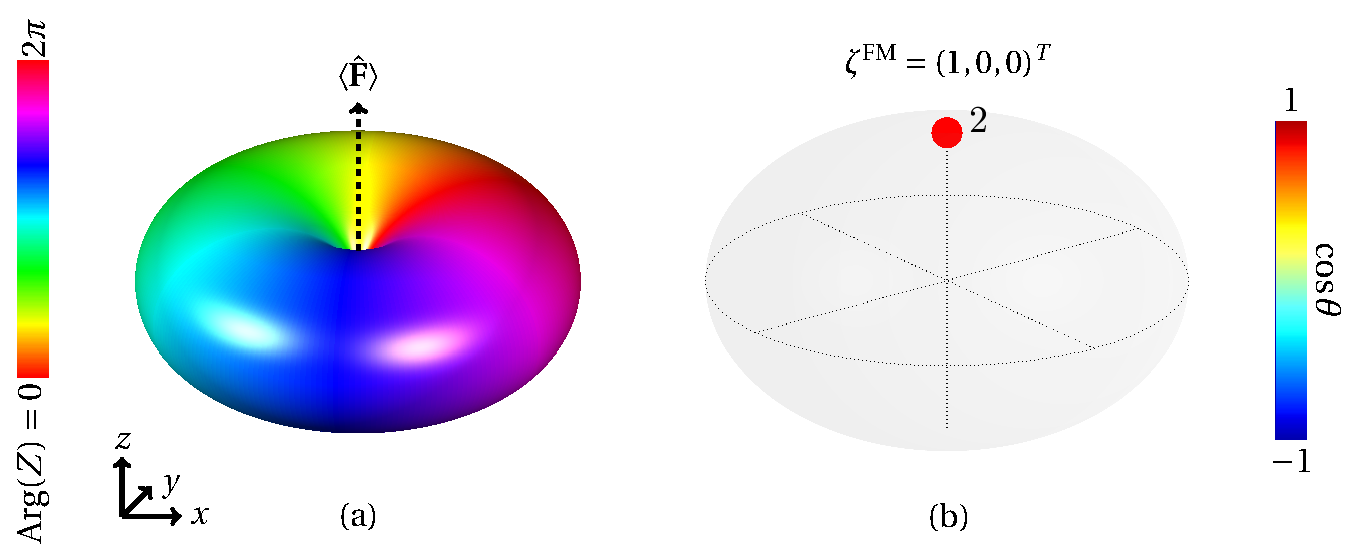
\includegraphics[width=\textwidth]
    {gfx/ch-groundStateSymmetries/spin-1-FM.pdf}
    \caption[Graphical representations of the spin-1 ferromagnetic ground
    state]{\label{fig: spin-1-FM-graph}Graphical representation of the spin-1
    ferromagnetic phase, with the representative spinor given by
    Eq.~\eqref{eq: spin-1-FM-rep-spinor}.
    (a): Spherical harmonic representation, where the black dashed arrow
    represents the direction of the condensate magnetisation.
    (b): Majorana representation, where the colour of the points represent
    \(\cos\theta = (1-|z|^2)/(1+|z|^2)\) and a number next to a point represents
    the root when the polynomial \(P^{(1)}(z)\) has an \(n\)-multiple root.}
\end{figure}
We see that the ferromagnetic order parameter has an \(\text{SO}(2)\) symmetry
about the direction of magnetisation, which in this case is the \(z\)-axis.
The order parameter space, which describes the symmetries associated with the
order parameter of the system, is \(\mathcal{M}_\text{FM}
= {\text{SO}(3)}_{\hat{\vb{F}}, \tau}\), i.e.,
the full 3D rotation group, where \(\tau\) and \(\hat{\vb{F}}\) denote
contributions to the symmetry from the global phase and spin, respectively.

\subsection{Polar phase}
Now consider the case of \(c_1 > 0\), typically referred to as polar (or
antiferromagnetic) interactions.
Then, Eq.~\eqref{eq: spin-1-int-energy} becomes minimised by having the spin
magnitude vanish \(\spinmag=0\).
For this case, the ground state is called polar, with a representative
spinor given as
\begin{equation}\label{eq: EAP-spinor}
    \zeta^\mathrm{EAP} = \mqty(0 \\ 1 \\ 0).
\end{equation}
Similar to the FM case, a general polar wave function is constructed as
\begin{equation}\label{eq: polar-representative-spinor}
    \psi^\mathrm{P} =
    \sqrt{n}e^{i\tau}U(\alpha, \beta, \gamma)\zeta^\mathrm{EAP} =
    \sqrt{n}e^{i\tau}\mqty(
    -\frac{e^{-i\alpha}}{\sqrt{2}}\sin\beta \\
    \cos\beta \\
    \frac{e^{i\alpha}}{\sqrt{2}}\sin\beta
    ).
\end{equation}
It is also often useful to characterise the polar state using the condensate
phase and an unoriented unit vector, \(\hat{\vb{d}} \equiv (d_x, d_y, d_z)\),
referred to as the nematic director~\cite{Ruostekoski2003}.
A wave function in this representation is given as
\begin{align}
    \psi^\mathrm{P} = \frac{\sqrt{n}e^{i\tau}}{\sqrt{2}}
    \mqty(-d_x + id_y \\ \sqrt{2}d_z \\ d_x + id_y).
\end{align}
The nematic director can, in the absence of a magnetic field, be used to
distinguish between the state given in Eq.~\eqref{eq: EAP-spinor} and an
alternative representative spinor of
\begin{align}\label{eq: EPP-polar}
    \zeta^\text{EPP} = \frac{1}{\sqrt{2}}\mqty(1 \\ 0 \\ 1).
\end{align}
The former has the nematic director aligned with the \(z\)-axis, and is
typically referred to as the easy-axis polar (EAP) phase.
The latter instead has the nematic director perpendicular to the \(z\)-axis,
and is either referred to as the easy-plane polar (EPP) phase or the
antiferromagnetic phase.
Throughout this thesis we shall prefer the term EPP when describing an
unmagnetised polar spinor of the form of Eq.~\eqref{eq: EPP-polar}.

Both the spherical harmonic and Majorana representations of the EAP and EPP
polar ground states are shown in Fig.~\ref{fig: spin-1-polar-graph}.
\begin{figure}
    \centering
    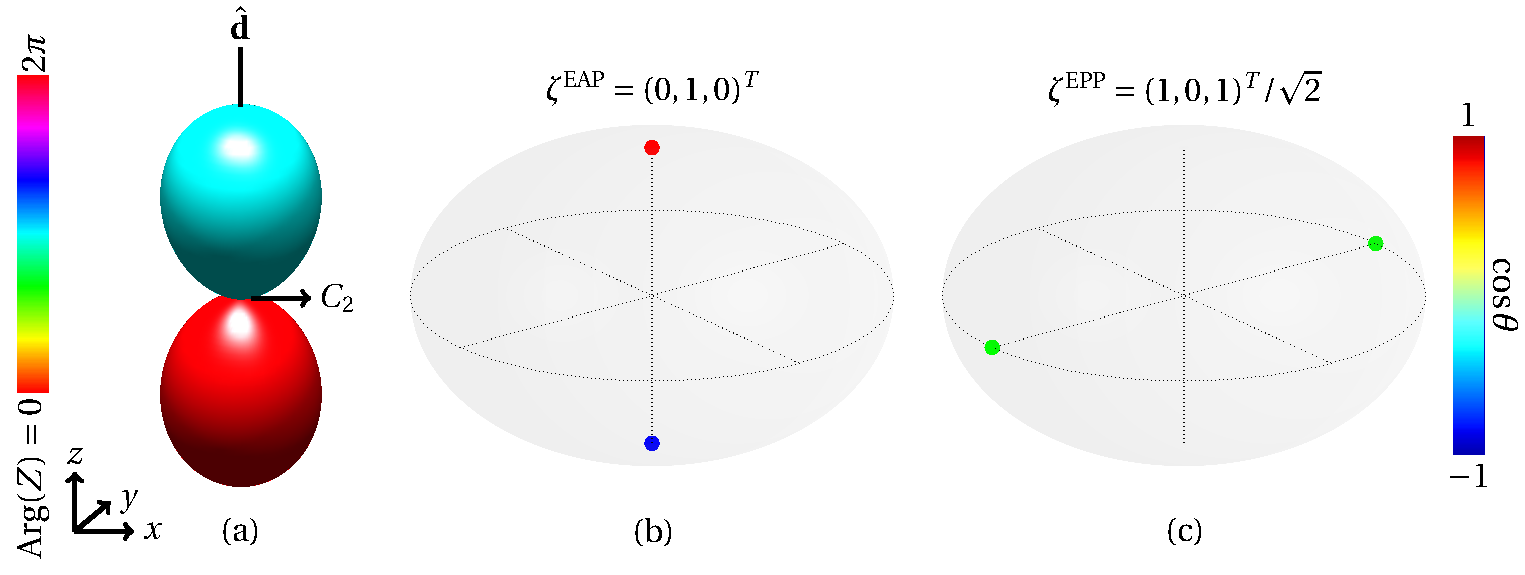
\includegraphics[width=\textwidth]
    {gfx/ch-groundStateSymmetries/spin-1-polar.pdf}
    \caption[Graphical representations of the spin-1 easy-axis polar and
    easy-plane polar ground states]{\label{fig: spin-1-polar-graph}Graphical
    representation of the EAP and EPP polar ground states.
    (a): Spherical harmonic representation of the EAP phase, with the
    representative spinor given as \(\zeta^\mathrm{P}={(0, 1, 0)}^T\).
    The nematic director \(\hat{\vb{d}}\) is aligned with the \(z\)-axis.
    Note that the EPP phase looks equivalent, but with the nematic director
    now laying in the \(xy\)-plane.
    The order parameter remains unchanged about \(\pi \) rotations about the
    \(C_2\) axis coupled with a \(\pi \) change of the condensate phase as
    \(\left(\hat{\vb{d}}, \tau\right) \rightarrow
    \left(-\hat{\vb{d}}, \tau+\pi\right)\).
    (b) and (c): Majorana representation of the EAP and EPP phase,
    respectively.}
\end{figure}
The polar state is distinguished by two nematic lobes which have a \(\pi \)
phase difference, hence the name polar.
These lobes are aligned along an axis of symmetry given by the nematic director,
\(\hat{\vb{d}}\).
In the above figure, the EPP phase is distinguished from the EPP phase by having
the nematic director lay in the \(xy\)-plane.
There is a further axis of symmetry about the \(C_2\) axis, about which \(\pi \)
rotations preserve the symmetry, but not the phase.
It can be seen that the order parameter will remain invariant under a change of
\(\zeta\left(\hat{\vb{d}}, \tau\right) \rightarrow
\zeta\left(-\hat{\vb{d}}, \tau + \pi\right)\).
The corresponding order parameter space is given as \(\mathcal{M} =
\left[S^2_{\hat{\vb{F}}} \cross {U(1)}_\tau\right] /
{({\mathbb{Z}}_2)}_{\hat{\vb{F}}, \tau} \)~\cite{Kawaguchi2012}.
Note that the \(\mathbb{Z}_2\) factor in the order parameter space arises from
the fact that the polar order parameter described in
Eq.~\eqref{eq: polar-representative-spinor} remains invariant under the
transformation described above.

\subsection{Ground states in the presence of magnetic fields}
The presence of an external magnetic field drastically changes the ground state
phase diagram of the spin-1 system.
\begin{figure}
    \centering
    \begin{tikzpicture}
        \node[anchor=south west, inner sep=0] (sodium) at (0, 0)
        {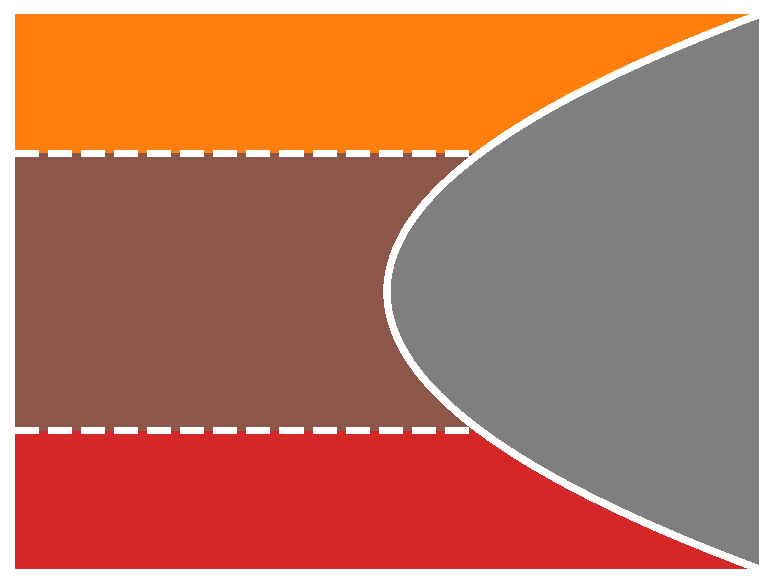
\includegraphics[width=0.38\textwidth]
            {gfx/ch-groundStateSymmetries/ground_states_polar_int_spin1.pdf}};
        \node[anchor=south west, inner sep=0] (rubidium) at (8, 0)
        {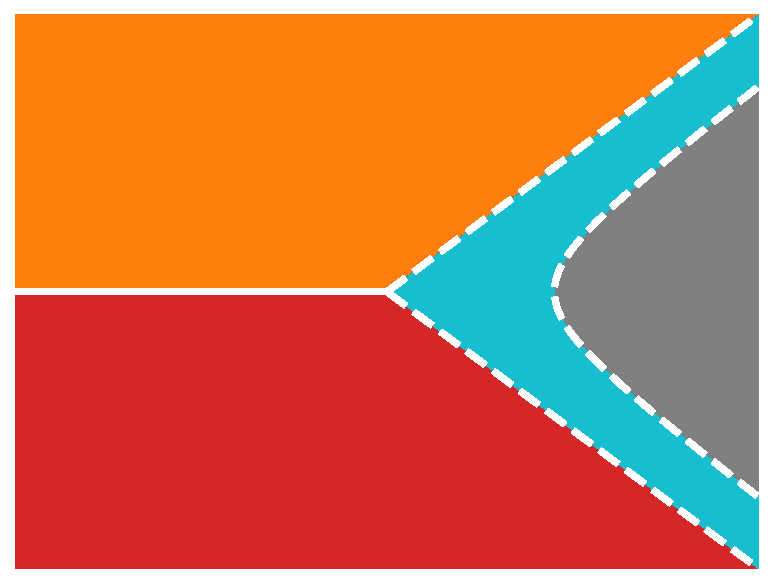
\includegraphics[width=0.38\textwidth]
            {gfx/ch-groundStateSymmetries/ground_states_fm_int_spin1.pdf}};

        \begin{scope}[x={($0.1*(sodium.south east)$)},
                y={($0.1*(sodium.north west)$)}]
            \draw[->, thick] (0,5)--(10.3,5) node[right]{\(\frac{q}{c_1n}\)};
            \draw[->, thick] (4.97,0)--(4.97,10.3) node[above]
                {\(\frac{p}{c_1n}\)};
            \draw[-] (6.1, 4.8) -- (6.1, 5.2);
            \node[anchor = south west] at (6.5, 3)
            {\scriptsize $p^2=2c_1nq$};
            \draw[->, thick] (6.6, 3.1) -- (6.25,2.55);
            \node at (4.8, 7.75) {\scriptsize \(1\)};
            \node at (4.7, 2.25) {\scriptsize \(-1\)};
            \node at (6.1, 4.5) {\scriptsize 1/2};
            \node[anchor=south west] at (0.5, 8.2)
            {\textcolor{white}{Ferromagnetic (I)}};
            \node[anchor=south west] at (0.5, 0.5)
            {\textcolor{white}{Ferromagnetic (II)}};
            \node[anchor=south west] at (2, 4.9)
            {\textcolor{white}{Polar}};
            \node[anchor=south west] at (2.1, 3.8)
            {\textcolor{white}{(III)}};
            \node[anchor=south west] at (6.5, 4.9)
            {\textcolor{white}{Polar (IV)}};
            \node[anchor=south west] at (3.8, -1.5) {\large \(c_1 > 0\)};
        \end{scope}
        \begin{scope}[x={($0.1*(sodium.south east)$)},
                y={($0.1*(sodium.north west)$)}]
            \draw[->, thick] (19.3,5)--(24.5,5) node[right]
                {\(\frac{q}{|c_1|n}\)};
            \draw[->, thick] (19.3,0)--(19.3,10.3) node[above]
            {$\frac{p}{|c_1|n}$};
            \node[anchor=south west] at (19.2, 8.6)
            {\scriptsize $p^2=q^2-2|c_1|nq$};
            \draw[->, thick] (19.7, 8.8) -- (21.9, 6.2);
            \node[anchor=south west, inner sep=0, rotate=-38] at (19.3, 4.)
            {\scriptsize $p=-q$};
            \node[anchor=south west, inner sep=0, rotate=38] at (19.5, 5.3)
            {\scriptsize $p=q$};
            \node[anchor=south west, inner sep=0] at (21.7, 4.5)
            {\scriptsize $2$};
            \node[anchor=south west] at (14.8, 6.5)
            {\textcolor{white}{Ferromagnetic (I)}};
            \node[anchor=south west] at (14.8, 1.5)
            {\textcolor{white}{Ferromagnetic (II)}};
            \node[anchor=south west] at (20.1, 4.9)
            {\textcolor{white}{BA}};
            \node[anchor=south west] at (20.1, 3.8)
            {\textcolor{white}{(V)}};
            \node[anchor=south west] at (22.1, 4.9)
            {\textcolor{white}{Polar}};
            \node[anchor=south west] at (22.1, 3.8)
            {\textcolor{white}{(IV)}};
            \node[anchor=south west] at (18., -1.5) {\large \(c_1 < 0\)};
        \end{scope}
    \end{tikzpicture}
    \caption[Spin-1 ground state phase diagram]
    {\label{fig: GS-phase-diagram}Ground state phase diagrams of spin-1
        BECs for \(c_1 > 0\) (left) and \(c_1 < 0\) (right) interactions in a
        parameter space of \((p, q)\).
        Solid or dashed white lines represent discontinuous and continuous phase
        transitions, respectively.}
\end{figure}
Fig.~\ref{fig: GS-phase-diagram} shows the ground state phase diagram for spin-1
BECs with \(c_1 > 0\) (left) and \(c_1 < 0\) (right) in the presence of a
magnetic field.
The full derivation of the ground state phase diagram can be found in
reviews~\cite{Kawaguchi2012, Stamper-Kurn2013}.
There are five total ground states shown in Fig.~\ref{fig: GS-phase-diagram},
which are summarised in Table~\ref{tab: spin-1-ground-states}.

There exists a fully magnetised ferromagnetic state with \(\zeta={(1, 0, 0)}^T\)
and \(\langle\hat{F}_z\rangle=1\) (state I) or \(\zeta={(0, 0, 1)}^T\) and
\(\langle\hat{F}_z\rangle=-1\) (state II), depending on the sign of the linear
Zeeman shift \(p\).
A non-magnetised polar phase (state IV) arises with \(\zeta={(0, 1, 0)}^T\) and
\(\langle\hat{F}_z\rangle = 0\).
For polar interactions \(c_1 > 0\), there exists a partially-magnetised polar
phase (state III) with
\begin{equation}\label{eq: AFM-spinor}
    \zeta^\mathrm{PMP} = {\left(\sqrt{\frac{1 + p/(c_1n)}{2}}, 0,
    \sqrt{\frac{1 - p/(c_1n)}{2}}\right)}^T,
\end{equation}
and \(\langle\hat{F}_z\rangle = p/(c_1n)\).
At \(p=0\), this state transforms into the non-magnetised EPP phase given in
Eq.~\eqref{eq: EPP-polar}, equivalent to state IV with the nematic director in
the \(xy\)-plane.
As \(p \rightarrow \pm c_1n\) this state tends toward the ferromagnetic states
I or II, respectively.
Finally, a broken-axisymmetry (BA) phase (state V) occurs in a condensate with
\(c_1 > 0\) which has a spinor of the form
\begin{equation}
    \begin{aligned}
        \zeta^\text{BA}_{\pm 1} & =
        \frac{q \pm p}{2q}\sqrt{\frac{-p^2+q^2+2c_1nq}{2c_1nq}}, \\
        \zeta_0^\text{BA} & = \sqrt{\frac{(q^2-p^2)(-p^2-q^2+2c_1nq)}{4c_1nq^3}}.
    \end{aligned}
    \label{eq: BA-spinor}
\end{equation}
This corresponds to a magnetisation that tilts against the quantisation axis,
given by
\begin{equation}
    \langle\hat{F}_z\rangle = \frac{p(-p^2 + q^2 + 2qc_1n)}{2c_1nq^2}.
\end{equation}
These five ground states fully encapsulate the phase diagram of spin-1 BECs
in a magnetic field.

\begin{table}
    \centering
    \begin{tabular}{ccc}
        \toprule
        Ground state & Spinor, \(\zeta^T\) & \(\langle\hat{F}_z\rangle\) \\
        \midrule
        Ferromagnetic (I) & \((1, 0, 0)\) & 1 \\
        Ferromagnetic (II) & \((0, 0, 1)\) & -1 \\
        Polar (III) & \(\left(\sqrt{\frac{1 + p(c_1n)}{2}}, 0,
        \sqrt{\frac{1 - p(c_1n)}{2}}\right)\) & \(\frac{p}{c_1n}\) \\
        Polar (IV) & \((0, 1, 0)\) & 0 \\
        Broken-axisymmetry (V) & Eq.~\eqref{eq: BA-spinor} &
        \(\frac{p(-p^2+q^2+2qc_1n)}{2c_1nq^2}\) \\
        \bottomrule
    \end{tabular}
    \caption[Ground states arising in spin-1 BECs in the presence of magnetic
    fields]
    {\label{tab: spin-1-ground-states}Summary of the ground state phases in a
    spin-1 BEC with their respective spinors and magnetisation.}
\end{table}

The spherical harmonic representations of the partially-magnetised polar
(state III) and broken-axisymmetry (state V) phases are shown in
Fig.~\ref{fig: spin-1-magnetised-graph}.
\begin{figure}
    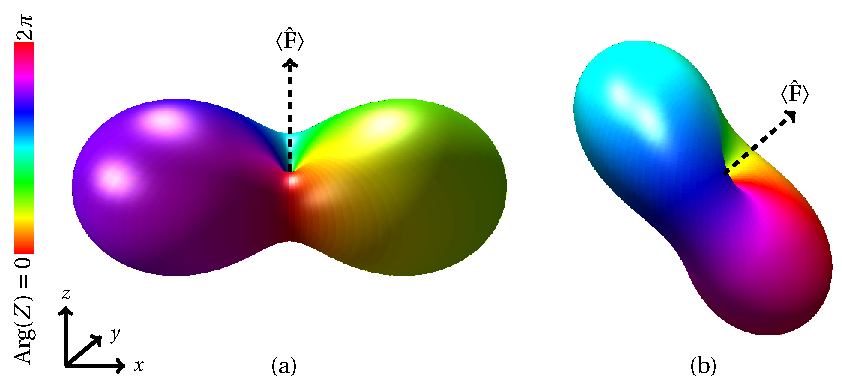
\includegraphics[height=0.4\textwidth, width=\textwidth]
    {gfx/ch-groundStateSymmetries/spin-1-magnetised.pdf}
    \caption[Spherical harmonic representation of the partially-magnetised polar
    and broken-axisymmetry phases in a spin-1 system]
    {\label{fig: spin-1-magnetised-graph}
    Spherical harmonics representation of both the partially-magnetised polar
    state and the broken-axisymmetry phase calculated using the appropriate
    representative spinor in Eq.~\eqref{eq: spherical-harmonics}.
    (a): The partially-magnetised polar state given by
    Eq.~\eqref{eq: AFM-spinor} with \(p \neq 0\).
    Note that for this state the direction of the spin vector is aligned with
    the applied magnetic field.
    (b): The broken-axisymmetry state given by Eq.~\eqref{eq: BA-spinor} with
    \(p, q \neq 0\).
    The direction of the spin vector is tilted away from the magnetic field
    axis, which is assumed to be along the \(z\)-axis.}
\end{figure}
For the partially-magnetised polar state, we see the effect of the linear
Zeeman shift breaking the symmetry of the spin when compared to the polar state
shown in Fig.~\ref{fig: spin-1-polar-graph}a.
The broken-axisymmetry phase is seen to tilt against the \(z\)-axis, which
arises due to the linear Zeeman shift, \(p\).

\section{Ground states of spin-2 BECs}\label{sec: ground-states-spin-2}
To find the ground states of a spin-2 system we follow a similar procedure to
the spin-1 case.
The interacting part of the spin-2 Hamiltonian reads (see
Sec.~\ref{subsec: spinor-interaction-hamiltonian})
\begin{align}
    E_\mathrm{int} = \frac{1}{2}\int c_0n^2 + c_1n^2\spinmag^2+c_2n^2|A_{00}|^2
    \dd^3\vb{r}.
\end{align}
As before, we assume a uniform ground state so that the density remains fixed.
Therefore, different ground states arise from the competition between the
spin-dependent, \(c_1\), and singlet-dependent, \(c_2\), interaction strengths.
The magnitude of the spin expectation is now defined in terms of the spin-2
spin vectors given in Eqs.~\eqref{eq: spin-2-spin-vectors}
and~\eqref{eq: spin-2-fz}, and the spin-singlet pair amplitude, \(A_{00}\),
given in Eq.~\eqref{eq: spin-singlet-duo}.

As in the spin-1 case, the energy of a given spinor in the absence of a magnetic
field is degenerate following the application of a global \(U(1)\) phase and an
\(SO(3)\) spin rotation.
In a spin-2 system, a general spin rotation is instead represented as a
\(5\times 5\) matrix of the form~\cite{Kawaguchi2012}
\begin{multline}\label{eq: spin-2-rotation-matrix}
    U(\alpha, \beta, \gamma) = \\
    \scalemath{0.90}{\mqty(
    e^{-2i(\alpha + \gamma)}C^4 & -2e^{-i(2\alpha+\gamma)}C^3S
    & \sqrt{6}e^{-2i\alpha}C^2S^2 & -2e^{-i(2\alpha-\gamma)}CS^3
    & e^{-2i(\alpha - \gamma)}S^4
    \\
    2e^{-i(\alpha+2\gamma)}C^3S & e^{-i(\alpha+\gamma)}C^2(C^2-3S^2)
    & -\sqrt{\frac{3}{8}}e^{-i\alpha}\sin 2\beta
    & -e^{-i(\alpha-\gamma)}S^2(S^2-3C^2) & -2e^{-i(\alpha-2\gamma)}CS^3
    \\
    \sqrt{6}e^{-2i\gamma}C^2S^2 & \sqrt{\frac{3}{8}}e^{-i\gamma}\sin 2\beta
    & \frac{1}{4}(1+3\cos 2\beta)
    & -\sqrt{\frac{3}{8}}e^{-i\gamma}\sin 2\beta
    & \sqrt{6}e^{2i\gamma}C^2S^2
    \\
    2e^{i(\alpha-2\gamma)}CS^3 & -e^{i(\alpha-\gamma)}S^2(S^2-3C^2)
    & \sqrt{\frac{3}{8}}e^{i\alpha}\sin 2\beta
    & e^{i(\alpha-\gamma)}C^2(C^2-3S^2) & -2e^{i(\alpha+2\gamma)}C^3S
    \\
    e^{2i(\alpha - \gamma)}C^4 & 2e^{i(2\alpha-\gamma)}CS^3
    & \sqrt{6}e^{2i\alpha}C^2S^2 & 2e^{i(2\alpha+\gamma)}C^3S
    & e^{2i(\alpha + \gamma)}C^4
    )},
\end{multline}
where \(S \equiv \sin(\beta/2)\) and \(C \equiv \cos(\beta/2)\).

The ground states of the spin-2 system in a parameter space of \((c_1, c_2)\)
are summarised in Fig.~\ref{fig: spin-2-ground-states}.
\begin{figure}
    \centering
    \begin{tikzpicture}
        \node[anchor=south west, inner sep=0] (diagram) at (0, 0)
        {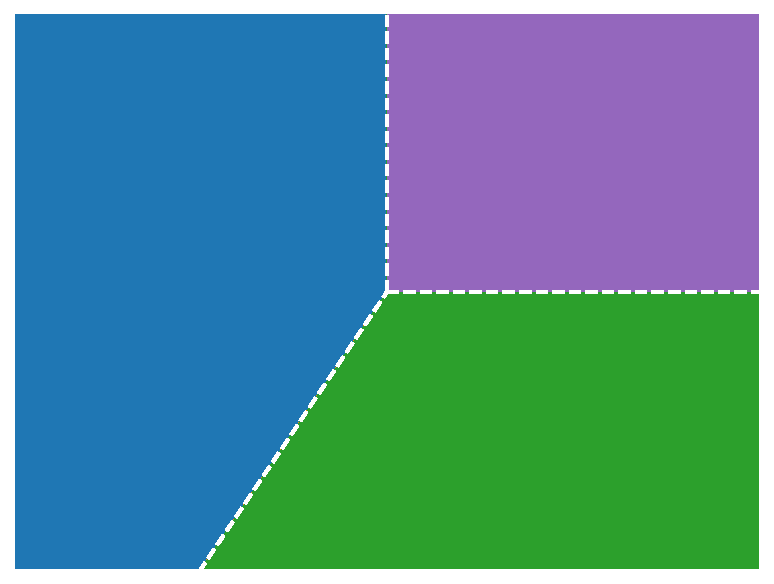
\includegraphics[width=0.5\textwidth]
            {gfx/ch-groundStateSymmetries/ground_states_spin2.pdf}};
        \begin{scope}[x={($0.1*(diagram.south east)$)},
                y={($0.1*(diagram.north west)$)}]
            \draw[->, thick, anchor=south west] (9.8, 5) -- (10.1, 5)
            node[right] {$c_1n$};
            \draw[->, thick, anchor=south west] (5, 9.7) -- (5, 10.1)
            node[above] {$c_2n$};
            \draw[-, thick, anchor=south west] (0.21, 5) -- (4.98, 5);
            \node at (7.5, 7) {\textcolor{white}{Cyclic}};
            \node at (2.5, 7) {\textcolor{white}{Ferromagnetic}};
            \node at (7, 2) {\textcolor{white}{Nematic}};
            \node[anchor=south east] at (5, 5) {\textcolor{white}{0}};
            \node[anchor=south west, rotate=53] at (2.7, 0.7)
            {\textcolor{white}{\(c_2n=20c_1n\)}};
        \end{scope}
    \end{tikzpicture}
    \caption[Spin-2 ground state phase diagram]
    {\label{fig: spin-2-ground-states}Ground state phase diagram for
        spin-2 BECs in a parameter space of \((c_1, c_2)\) in the absence of a
        magnetic field.
        White dashed lines indicate a first-order phase transition region
        between the phases.}
\end{figure}
In the following subsections we shall discuss each phase individually, along
with their respective graphical representations and order parameter spaces.
Note, for the case of \(c_1, c_2 < 0\), there is a competition between
the ferromagnetic and nematic phases.
For this case, the energy functional is minimised by either having maximal spin
density and \(|A_{00}|^2 = 0\) as in the ferromagnetic phase, or by having
minimal spin density and \(|A_{00}|^2 = 1/5\) as in the nematic phase, which
leads to a phase boundary at \(c_2n=20c_1n\) (see below).

\subsection{Ferromagnetic phase}
If we first consider \(c_1 < 0\) and \(c_2 > 0\), then the energy functional is
minimised when the spin density is maximised, \(\spinmag=2\),
and the singlet-duo amplitude is minimised, \(|A_{00}|=0\).
This state is denoted as the spin-2 ferromagnetic phase, where \(\spinmag \) is
now \(\spinmag=2\) for this ground state, as opposed to \(\spinmag=1\) in the
spin-1 system.
Note that there exists a ferromagnetic state in a spin-2 BEC with
\(\spinmag=1\), but this state is not the ground state since the \(\spinmag=2\)
state has lower energy.
To avoid confusion, we refer to the ferromagnetic state with \(\spinmag=2\) as
the \(\text{FM}_2\) state, and the state with \(\spinmag=1\) as the
\(\text{FM}_1\) state.
It should be noted, however, that the \(\text{FM}_1\) state can remain stable in
certain situations, such as in the cores of vortices (see
Chapter~\ref{chap: spin-2}).
The representative spinors for the spin-2 ferromagnetic states have the form
\begin{equation}\label{eq: FM2-FM1-spinors}
    \zeta^{\text{FM}_2} = \mqty(1 \\ 0 \\ 0 \\ 0 \\ 0), \qquad
    \zeta^{\text{FM}_1} = \mqty(0 \\ 1 \\ 0 \\ 0 \\ 0).
\end{equation}
Following the same procedure as the spin-1 case, applying a general spin
rotation \(U(\alpha, \beta, \gamma)\) with a global phase \(\tau \) and
condensate density \(n\) yields the general \(\text{FM}_2\) wave function which
describes all ferromagnetic states that have \(\spinmag=2\) in a spin-2 system:
\begin{equation}\label{eq: FM-2-representative-spinor}
    \psi^{\text{FM}_2} = \sqrt{n}e^{i(\tau-2\gamma)}\mqty(
    e^{-2i\alpha} \cos^4\frac{\beta}{2} \\
    2e^{-i\alpha}\cos^3\frac{\beta}{2}\sin \frac{\beta}{2} \\
    \sqrt{6} \cos^2\frac{\beta}{2} \sin^2\frac{\beta}{2} \\
    2e^{i\alpha}\cos\frac{\beta}{2} \sin^3\frac{\beta}{2} \\
    e^{2i\alpha} \sin^4\frac{\beta}{2}
    ).
\end{equation}
Equivalently, the general spinor for the \(\text{FM}_1\) phase is given as
\begin{align}
    \zeta^{\text{FM}_1} = \sqrt{n}e^{i(\tau - \gamma)}\mqty(
        -2e^{-2i\alpha}\cos^3\frac{\beta}{2}\sin\frac{\beta}{2} \\
        e^{-i\alpha}\cos^2\frac{\beta}{2}\left[\cos^2\frac{\beta}{2}^2
            -3\sin^2\frac{\beta}{2}\right] \\
        \sqrt{\frac{3}{8}}\sin2\beta \\
        -e^{i\alpha}\sin^2\frac{\beta}{2}\left[\sin^2\frac{\beta}{2}
            -3\cos^2\frac{\beta}{2}\right] \\
        2e^{2i\alpha}\cos\frac{\beta}{2}\sin^3\frac{\beta}{2}
    ).
\end{align}

Fig.~\ref{fig: spin-2-FM-graph} shows the spherical harmonic and Majorana
representations of the spin-2 ferromagnetic ground states.
\begin{figure}
    \centering
    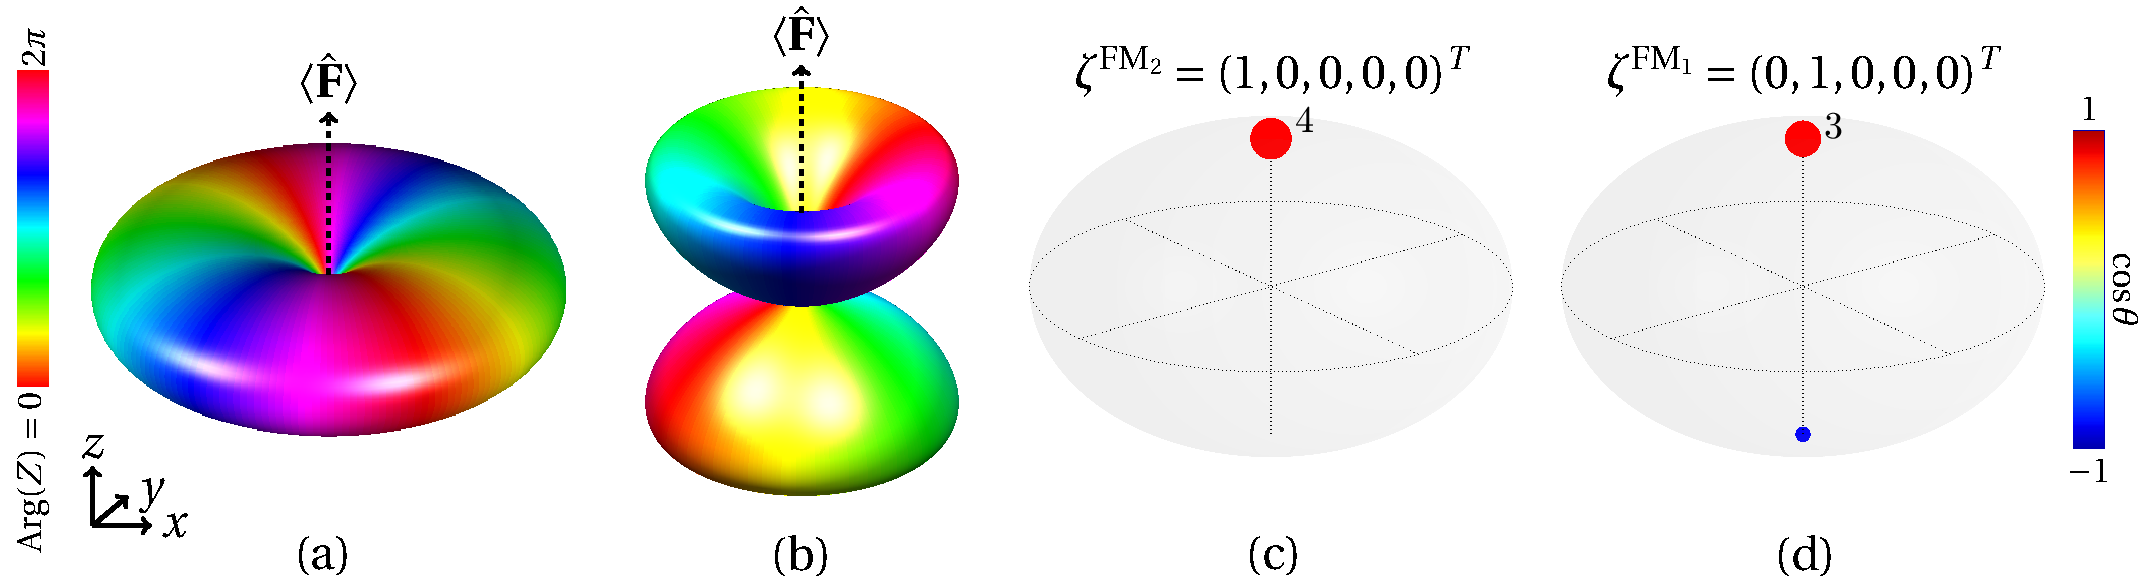
\includegraphics[width=\textwidth]
    {gfx/ch-groundStateSymmetries/spin-2-FM.pdf}
    \caption[Graphical representations of both spin-2 ferromagnetic states]
    {\label{fig: spin-2-FM-graph}Spherical harmonic and Majorana
    representations of the spin-2 ferromagnetic ground states, with
    representative spinors given in Eq.~\eqref{eq: FM2-FM1-spinors}.
    (a) and (b): Spherical harmonic representation for the ferromagnetic states
    with \(\spinmag=2\) and \(\spinmag=1\), respectively, where the dashed line
    represents the direction of the magnetisation.
    (c) and (d): Equivalent Majorana representations.}
\end{figure}
It is clear from Figs~\ref{fig: spin-2-FM-graph}a, b that the ferromagnetic
order parameters have the same \(\text{SO}(2)\) symmetry about the direction of
the magnetisation as in the spin-1 case.
However, the difference between the \(\text{FM}_2\) phase of the spin-2 system
and the FM phase of the spin-1 system is apparent in the phase: the
\(\text{FM}_2\) state winds by \(4\pi \) about the spherical harmonic as opposed
to \(2\pi \) (see Fig.~\ref{fig: spin-1-FM-graph}).
Therefore, the order parameter space of the \(\text{FM}_2\) phase is  slightly
different, and given as
\(\mathcal{M}_{\text{FM}_2} = {\text{SO}(3)}_{\hat{\vb{F}}, \tau} /
{(\mathbb{Z}_2)}_{\hat{\vb{F}}, \tau}\).
The \({(\mathbb{Z}_2)}_{\hat{\vb{F}}, \tau}\) factor arises from the double
winding of the condensate phase seen above.

\subsection{Nematic phases}
Instead, let us now consider the case of \(c_1 > 0\) and \(c_2 < 0\).
We see that the energy functional is minimised when the spin is minimised,
\(\spinmag = 0\), but the singlet-duo amplitude is maximised,
\(|A_{00}|^2 = 1/5\).
Such a state is called nematic, and takes two forms: the uniaxial nematic (UN)
or biaxial nematic (BN), depending on the sign of the quadratic Zeeman shift,
\(q\).
A representative spinor for the UN state, where the nematic director
\(\hat{\vb{d}}\) is aligned along the \(z\)-axis, is given as
\begin{align}\label{eq: UN-spinor}
    \zeta^\mathrm{UN} = \mqty(0 \\ 0 \\ 1 \\ 0 \\ 0),
\end{align}
and a representative spinor for the BN state reads
\begin{align}\label{eq: BN-spinor}
    \zeta^\mathrm{BN} &= \frac{1}{\sqrt{2}}\mqty(1 \\ 0 \\0 \\ 0 \\ 1).
\end{align}
Applying a general spin rotation and condensate phase leads to the general wave
functions for the UN and BN states, respectively, as
\begin{align}\label{eq: UN-representative-spinor}
    \psi^\mathrm{UN} = \frac{\sqrt{6n}}{4}e^{i\tau}\mqty(
    e^{-2i\alpha} \sin^2\beta \\
    -2e^{-i\alpha} \sin\beta \cos\beta \\
    \sqrt{\frac{2}{3}}(3\cos^2\beta - 1) \\
    2e^{i\alpha} \sin\beta \cos\beta \\
    e^{2i\alpha} \sin^2\beta
    ),
\end{align}
\begin{align}\label{eq: BN-representative-spinor}
    \psi^\mathrm{BN} = \sqrt{\frac{n}{2}}e^{i\tau} \mqty(
    e^{-2i\alpha}\left[\left(1 - \frac{1}{2}\sin^2\beta\right)\cos 2\gamma
        - i\cos\beta\sin 2\gamma\right] \\
    e^{-i\alpha}\sin\beta(\cos\beta\cos 2\beta - i\sin 2\gamma) \\
    \sqrt{\frac{3}{2}}\sin^2\beta \cos 2\gamma \\
    -e^{i\alpha}\sin\beta(\cos\beta\cos 2\gamma + i\sin 2\gamma) \\
    e^{2i\alpha}\left[\left(1 - \frac{1}{2}\sin^2\beta\right)\cos 2\gamma
        + i\cos\beta\sin 2\gamma\right]
    ).
\end{align}
In the absence of a magnetic field, these two states are degenerate.
However, a quadratic Zeeman shift, \(q\), can be used to manipulate the system
into choosing one or the other, since the energies of each ground state now
change (energetic stability of these states is discussed in
Sec.~\ref{subsec: UN-BN-defects}).

The spherical harmonics and Majorana representation of both nematic states are
plotted in Fig.~\ref{fig: nematic-graph}.
\begin{figure}
    \centering
    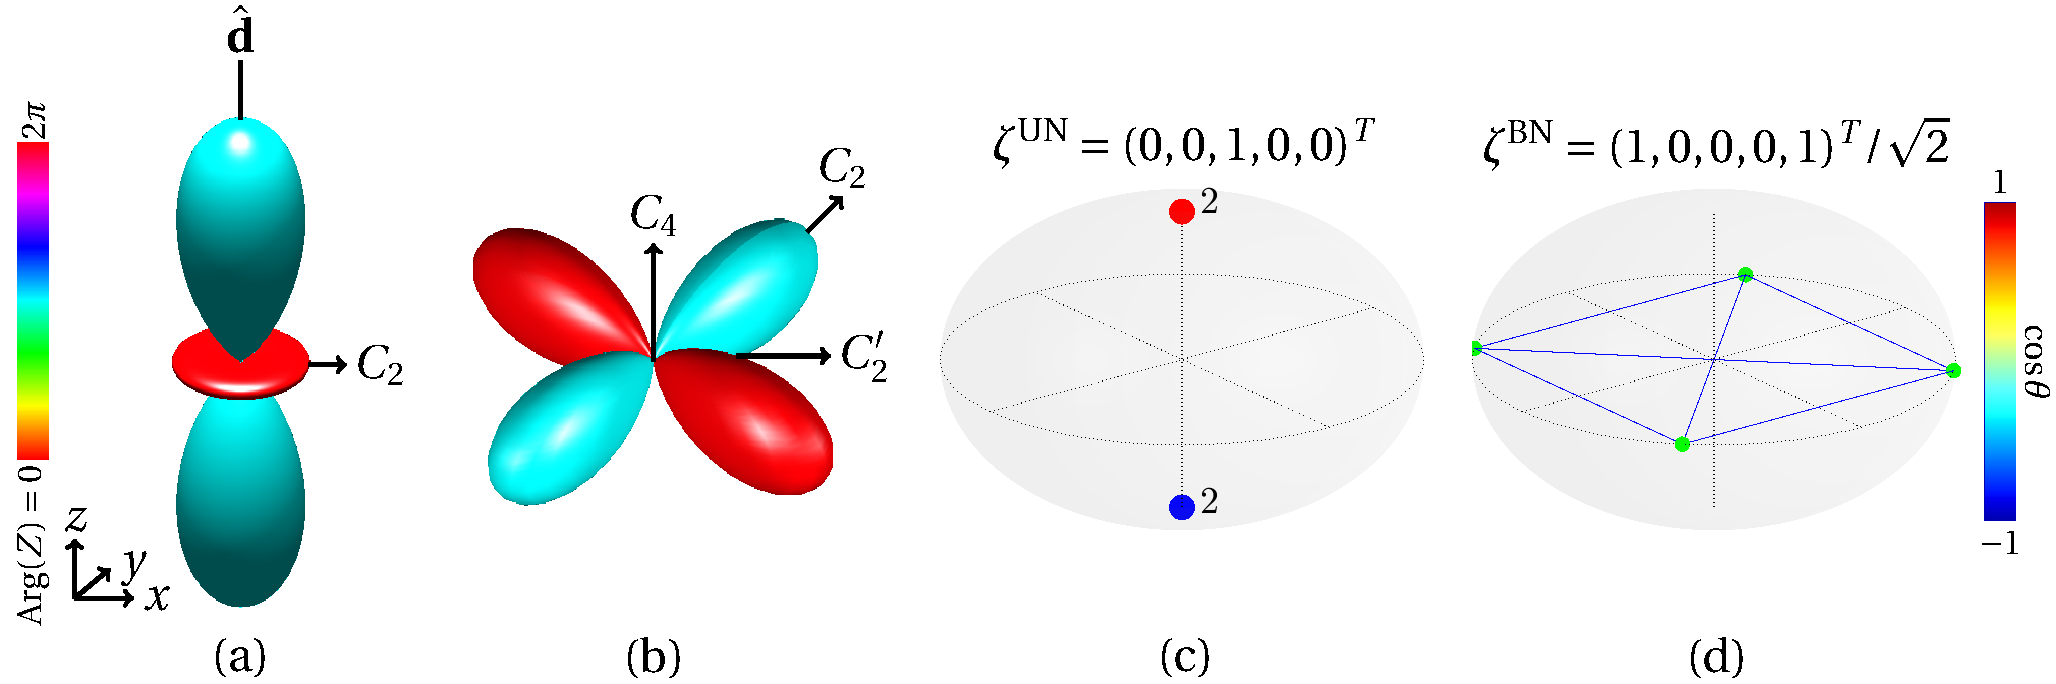
\includegraphics[width=\textwidth]
    {gfx/ch-groundStateSymmetries/spin-2-nematic.pdf}
    \caption[Graphical representations of the spin-2 nematic ground states]
    {\label{fig: nematic-graph}Spherical harmonic and Majorana representations
    of the spin-2 nematic ground states.
    (a): Spherical harmonic representation of the uniaxial nematic spinor given
    in Eq.~\eqref{eq: UN-spinor} where \(\hat{\vb{d}}\) is the nematic director.
    The order parameter exhibits a two-fold symmetry about the \(C_2\) axis.
    (b) Spherical harmonic representation of the biaxial nematic state given by
    Eq.~\eqref{eq: BN-spinor} which has a four-fold symmetry about the \(C_4\)
    axis, and two additional two-fold symmetries about the \(C_2, C_2'\) axes.
    (c) and (d): Equivalent Majorana representations.}
\end{figure}
The UN phase is seen to differ slightly from the polar phase of spin-1 (see
Fig.~\ref{fig: spin-1-polar-graph}a) in that the nematic lobes have the
same phase.
This implies that a \(\pi \) spin rotation about the \(C_2\) axis leaves the
order parameter unchanged, and no appropriate transformation of the condensate
phase has to occur.
In addition, this order parameter also has an \(SO(2)\) symmetry about the
nematic director.
The order parameter space for this phase is then calculated as
\(\left[S^2_{\hat{\vb{F}}} \cross {U(1)}_\tau\right]
/ {({\mathbb{Z}}_2)}_{\hat{\vb{F}}} \).
This is identical to the polar phase of the spin-1 BEC, except now the
\({(\mathbb{Z}_2)}_{\hat{\vb{F}}}\) arises only from the condensate spin due to
the nematic lobes having the same phase.
The BN phase, shown in Fig.~\ref{fig: nematic-graph}b, breaks the
\(\text{SO}(2)\) symmetry due to the perpendicular nematic lobes, which have a
\(\pi \) phase difference.
The symmetry of the order parameter is preserved under \(\pi/4\) rotations
about the \(C_4\) axis and \(\pi\) rotations about both the \(C_2\) and \(C_2'\)
axes.
The order parameter space for this phase is calculated as
\(\left[{\text{U}(1)}_\tau \cross {\text{SO}(3)}_{\hat{\vb{F}}}\right]
/ {(\text{D}_4)}_{\hat{\vb{F}}, \tau}\), where \(\text{D}_4\) is the fourth
dihedral group~\cite{Kobayashi2012}.

\subsection{Cyclic phase}
Now consider \(c_1, c_2 > 0\).
The energy functional is minimised when both the spin magnitude and singlet-duo
amplitude is minimised: \(\spinmag = 0, |A_{00}|^2=0\).
Such a state is referred to as the cyclic state and has the representative
spinor
\begin{equation}
    \zeta^{\text{C}_1} = \frac{1}{2}\mqty(1 \\ 0 \\ i\sqrt{2} \\ 0 \\ 1).
    \label{eq: C-1-spinor}
\end{equation}
The general wave function is calculated as
\begin{equation}\label{eq: general-cyclic-wfn}
    \psi^\mathrm{C} = \frac{\sqrt{n}}{2}e^{i\tau} \mqty(
    e^{-2i(\alpha+\gamma)}C^4 + 2i\sqrt{3}e^{-2i\alpha}C^2S^2
    + e^{-2i(\alpha-\gamma)}S^4
    \\
    2e^{-i(\alpha+2\gamma)}C^3S - \frac{\sqrt{3}}{2}ie^{-i\alpha}\sin 2\beta
    - 2e^{-i(\alpha-2\gamma)}CS^3
    \\
    \sqrt{6}e^{-2i\gamma}C^2S^2 + i\frac{\sqrt{2}}{4}(1+3\cos 2\beta)
    + \sqrt{6}e^{2i\gamma}C^2S^2
    \\
    2e^{i(\alpha-2\gamma)}CS^3 + \frac{\sqrt{3}}{2}ie^{i\alpha}\sin 2\beta
    - 2e^{i(\alpha+2\gamma)}C^3S
    \\
    e^{2i(\alpha-\gamma)}S^4 + 2i\sqrt{3}e^{2i\alpha}C^2S^2
    + e^{2i(\alpha+\gamma)}C^4
    ).
\end{equation}
In addition to the three-component cyclic state, there is also a two-component
cyclic state that is useful for understanding the general cyclic state:
\begin{equation}
    \zeta^{\text{C}_2} = \frac{1}{\sqrt{3}}\mqty(1  \\ 0 \\ 0 \\ \sqrt{2} \\ 0),
    \label{eq: C-2-spinor}
\end{equation}
which is obtained from Eq.~\eqref{eq: C-1-spinor} via the spin
rotation~\cite{Kawaguchi2012}
\begin{equation}\label{eq: cyclic-spin-rotation}
    \zeta^{\text{C}_2} = -ie^{i\frac{\pi}{4}\hat{F}_z}
    \exp\left[i\frac{\hat{F}_x-\hat{F}_y}{\sqrt{2}}
        \arccos{\left(\frac{1}{\sqrt{3}}\right)}\right]\zeta^{\text{C}_1}.
\end{equation}

The spherical harmonic and Majorana representations of both orientations of the
cyclic state are plotted in Fig.~\ref{fig: cyclic-graph}.
\begin{figure}
    \centering
    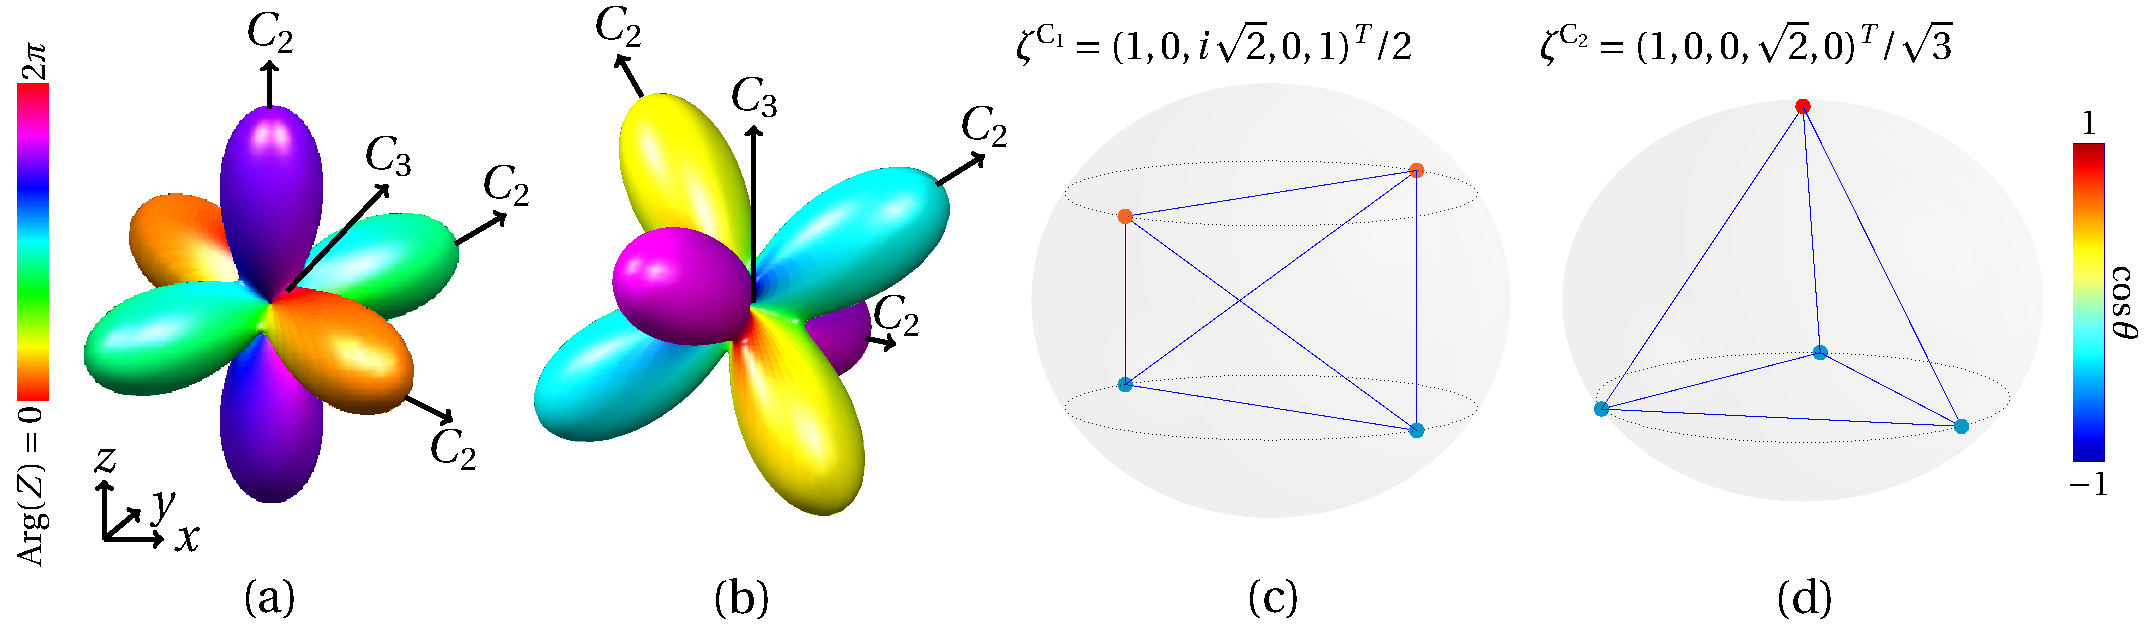
\includegraphics[width=\textwidth]
    {gfx/ch-groundStateSymmetries/spin-2-cyclic.pdf}
    \caption[Graphical representations of two different orientations of the
    cyclic ground state.]
    {\label{fig: cyclic-graph}Spherical harmonic and Majorana representations of
    two different orientations of the spin-2 cyclic ground state.
    (a): Cyclic state given by Eq.~\eqref{eq: C-1-spinor} which has a two- and
    three-fold symmetry about the \(C_2, C_3\) axes, respectively.
    (b): Alternative, two-component cyclic state, given by
    Eq.~\eqref{eq: C-2-spinor} which is obtained from (a) by the spin rotation
    given in Eq.~\eqref{eq: cyclic-spin-rotation}.
    (c) and (d): Equivalent Majorana representations.}
\end{figure}
The cyclic order parameter has the symmetry of a tetrahedron, where each nematic
lobe has a two-fold symmetry about each \(C_2\) axis.
Furthermore, the order parameter has a three-fold symmetry about the \(C_3\)
axis, of which \(2\pi/3\) rotations about this axis preserve the symmetry of the
order parameter.
In Fig.~\ref{fig: cyclic-graph}a, this axis is the \((1, 1, 1)\)-axis, whereas
in Fig.~\ref{fig: cyclic-graph}b the three-fold axis of symmetry is the
\(z\)-axis.
The order parameter space of the cyclic phase can be written as
\(\left[{\text{U}(1)}_\tau \cross {\text{SO}(3)}_{\hat{\vb{F}}}\right]
/ \text{T}_{\hat{\vb{F}}, \tau}\)~\cite{Kawaguchi2012}, where
\(\text{T}_{\hat{\vb{F}}, \tau}\) is the tetrahedral group~\cite{Kobayashi2012}.

\section{Topologically stable defects in spinor BECs}
Due to their rich phase diagrams discussed in the previous sections, spinor BECs
give rise to multiple different types of topological defects.
Such defects range from vortices, both singular~\cite{Yip1999,Isoshima2002,
Mizushima2002, Sadler2006,Semenoff2007,Lovegrove2012,Lovegrove2016,
Borgh2016,Weiss2019,Xiao2021,Xiao2022}, including singular
fractional vortices~\cite{Leonhardt2000, Zhou2003,Ji2008,Seo2015,Semenoff2007,
Kobayashi2009,Lovegrove2012, Lovegrove2016,Borgh2016,Borgh2017,Xiao2021,
Xiao2022}, and nonsingular~\cite{Ohmi1998, Ho1998, Mizushima2002a,
Martikainen2002, Leanhardt2003, Mizushima2004, Choi2012, Choi2012a,
Lovegrove2014,Weiss2019}, to point defects such as monopoles~\cite{Stoof2001,
Savage2003,Ruostekoski2003, Pietila2009,Ray2014,Ray2015,Ollikainen2017,
Mithun2022}.

The types of topologically stable defects within a given system can be
found from a group-theoretical approach using homotopy theory~\cite{Mermin1979,
Kawaguchi2012}.
The theory states that the \(n\)th homotopy group, \(\pi_n\), classifies
topological excitations with dimension of homotopy \(n\), where
\(n = d - \nu - 1\) for singular excitations and \(n=d - \nu \) for nonsingular
excitations~\cite{Kobayashi2012}.
Here, \(d\) and \(\nu \) describe the dimensionality of the system and the
dimensionality of the excitation, respectively.
To calculate whether a given defect is stable in a particular system, one needs
to first find the relevant order parameter space, \(\mathcal{M}\), that
describes the symmetries associated with the order parameter of that system.
Then, calculating a given homotopy group, \(\pi_n(\mathcal{M})\), states whether
the types of topological defects described by \(\pi_n\) are stable in that order
parameter space.
For example, given an order parameter space \(\mathcal{M}\), one can calculate
whether point defects (\(n=2\)) are stable within the system by seeing if
\(\pi_2(\mathcal{M}) \neq 0\).
Homotopy groups and the topological excitations they describe are listed in
Table~\ref{tab: homotopy-groups}~\cite{Kawaguchi2012}.
\begin{table}
    \centering
    \begin{tabular}{ccc}
        \toprule
        \(\pi_n\) & Defects & Solitons \\
        \midrule
        \(\pi_1 \) & Vortices & Nonsingular domain walls \\
        \(\pi_2 \) & Monopoles & 2D Skyrmions \\
        \(\pi_3 \) &  & (3D) Skyrmions, knots \\
        \bottomrule
    \end{tabular}
    \caption[Homotopy groups and the topological excitations they describe]
    {\label{tab: homotopy-groups}A list of different homotopy groups
    and the corresponding topological defects/solitons they
    describe~\cite{Kawaguchi2012}.}
\end{table}

In this section, we list the order parameter space for each ground state
in both spin-1 and spin-2 systems, which we then use to deduce the possible
stable defect structures in each phase by calculating the homotopy groups of the
space.

\subsection{Homotopy groups for a spin-1 system}
Recall that a spin-1 system has two phases in the absence of a magnetic field:
ferromagnetic and polar.
The order parameter space and the first three homotopy groups for these phases
are calculated and listed in
Table~\ref{tab: spin-1-homotopy-groups}~\cite{Mermin1979,Kawaguchi2012,
Kobayashi2012}.
\begin{table}
    \centering
    \begin{tabular}{ccccc}
        \toprule
        Spin-1 phase & \(\mathcal{M}\) & \(\pi_1\) & \(\pi_2\) & \(\pi_3\) \\
        \midrule
        Polar & \(\left[S^2_{\hat{\vb{F}}} \cross {U(1)}_\tau\right]
        / {({\mathbb{Z}}_2)}_{\hat{\vb{F}}, \tau} \)
        & \(\mathbb{Z}\) & \(\mathbb{Z}\)  & \(\mathbb{Z}\) \\
        Ferromagnetic & \({\text{SO}(3)}_{\hat{\vb{F}}, \tau}\)
        & \({\mathbb{Z}}_2\) & 0  & \(\mathbb{Z}\) \\
        \bottomrule
    \end{tabular}
    \caption[Order parameter spaces and first three homotopy groups for spin-1
    BECs]{\label{tab: spin-1-homotopy-groups}Spin-1 phases and their relative
    order parameter space, \(\mathcal{M}\) along with the corresponding first
    (\(\pi_1\)), second (\(\pi_2\)), and third (\(\pi_3\)) homotopy
    groups~\cite{Kobayashi2012}.
    Here, \(\hat{\vb{F}}\) and \(\tau \) indicate contributions from the
    condensate spin and phase, respectively.}
\end{table}

We start with the polar phase, with the representative spinor defined as in
Eq.~\eqref{eq: polar-representative-spinor}.
The first homotopy group is calculated to be the additive group of integers,
\(\pi_1(\mathcal{M}_\text{polar}) = \mathbb{Z}\), which indicates vortices are
stable and classified by integers within this phase.
It is worth noting that the first homotopy group for a scalar BEC system,
which has an order parameter space of \(\mathcal{M}_\text{scalar}
= \text{U}(1)\), is the same: \(\pi_1(\mathcal{M}_\text{scalar}) = \mathbb{Z}\).
However, due to the \({\mathbb{Z}}_2\) symmetry, the minimum unit of circulation
becomes half that of a scalar \(\text{U}(1)\) vortex, giving rise to what are
known as half-quantum vortices (HQVs)~\cite{Kawaguchi2012} (see
Sec.~\ref{sec: vortices-spin-1}).
In addition, the polar phase supports stable point defects since
\(\pi_2(\mathcal{M}_\text{UN}) = \mathbb{Z}\), where the point defects are
classified by integers.

The FM phase, described generally by Eq.~\eqref{eq: FM-representative-spinor},
has an order parameter space consisting of the full 3D rotation group:
\(\mathcal{M}_\text{FM} = {\text{SO}(3)}_{\hat{\vb{F}}, \tau}\).
This leads to a first homotopy group of \(\pi_1(\mathcal{M}_\text{FM})
= {\mathbb{Z}}_2\), which states that vortices are classified one of two ways in
this phase.
One class represents singular vortices and the other nonsingular, where the
vortex is classified by a fountain-like texture of the condensate spin vector
(see Sec.~\ref{sec: vortices-spin-1}).
Additionally, unlike the polar phase, the FM phase does not support stable point
defects since \(\pi_2(\mathcal{M}_\text{FM}) = 0\).

\subsection{Homotopy groups for a spin-2 system}\label{subsec: spin-2-homotopy}
As shown in Sec.~\ref{sec: ground-states-spin-2}, spin-2 BECs have a richer
phase diagram, and with that an even richer family of topological defects.
The order parameter spaces along with the first three homotopy groups are
given in Table~\ref{tab: spin-2-homotopy-groups}~\cite{Mermin1979,Kawaguchi2012,
Kobayashi2012}.
\begin{table}
    \centering
    \begin{tabular}{ccccc}
        \toprule
        Spin-2 phase & \(\mathcal{M}\) & \(\pi_1\) & \(\pi_2\) & \(\pi_3\) \\
        \midrule
        Uniaxial nematic & \(\left[S^2_{\hat{\vb{F}}} \cross {U(1)}_\tau\right]
        / {({\mathbb{Z}}_2)}_{\hat{\vb{F}}} \)
        & \(\mathbb{Z} \cross \mathbb{Z}_2\)
        & \(\mathbb{Z}\) & \(\mathbb{Z} \) \\
        Biaxial nematic & \(\left[{\text{U}(1)}_\tau \cross
        {\text{SO}(3)}_{\hat{\vb{F}}}\right]
        / {(\text{D}_4)}_{\hat{\vb{F}}, \tau}\)
        & \(\mathbb{Z} \cross_h {(\text{D}^\ast_4)}_{\hat{\vb{F}}}\) & 0
        & \(\mathbb{Z}\) \\
        Cyclic & \(\left[{\text{U}(1)}_\tau
        \cross {\text{SO}(3)}_{\hat{\vb{F}}}\right]
        / \text{T}_{\hat{\vb{F}}, \tau}\)
        & \(\mathbb{Z} \cross_h \text{T}_{\hat{\vb{F}}, \tau}\) & 0
        & \(\mathbb{Z}\) \\
        Ferromagnetic & \({\text{SO}(3)}_{\hat{\vb{F}}, \tau}
        / {({\mathbb{Z}}_2)}_{\hat{\vb{F}}, \tau}\)
        & \({\mathbb{Z}}_4\) & 0 & \(\mathbb{Z}\) \\
        \bottomrule
    \end{tabular}
    \caption[Order parameter spaces and first three homotopy groups for spin-2
    BECs]{\label{tab: spin-2-homotopy-groups}Spin-2 phases and their relative
    order parameter space, \(\mathcal{M}\), along with the corresponding first
    (\(\pi_1\)), second (\(\pi_2\)), and third (\(\pi_3\)) homotopy groups.
    Here, \(\hat{\vb{F}}\), \(\tau \) indicate contributions from the
    condensate spin and phase, respectively.
    Additionally, \(\text{D}_4\) and T represent the fourth dihedral and
    tetrahedral groups, respectively, and a \(\ast \) denotes a lift of that
    particular group~\cite{Mermin1979}.
    Finally, \(\cross_h\) is the \(h\)-product (see~\cite{Kobayashi2012} for
    details).}
\end{table}

Firstly, note that the order parameter space for the FM phase is slightly
different from the spin-1 case in that it is now divided by a
\({(\mathbb{Z}_2)}_{\hat{\vb{F}}, \tau}\) factor.
This contribution arises from the double winding of the condensate phase seen in
the spherical harmonic representation in Fig.~\ref{fig: spin-2-FM-graph}a.
The first homotopy group is also different, allowing now for an additional two
classes of line defects as \(\pi_1(\mathcal{M}_\text{FM}) = \mathbb{Z}_4\), but
the second and third homotopy groups are the same.

The UN phase has an identical order parameter space to the polar phase of a
spin-1 BEC, except now the \({(\mathbb{Z}_2)}_{\hat{\vb{F}}}\) factor arises
only from the condensate spin since the nematic lobes are no longer \(\pi \)
out of phase (see Fig.~\ref{fig: nematic-graph}a and
Fig.~\ref{fig: spin-1-polar-graph}b).
In addition, the first homotopy group differs slightly as now it reads
\(\pi_1(\mathcal{M}_\text{UN}) = \mathbb{Z} \cross
\mathbb{Z}_2\)~\cite{Kobayashi2012}, which allows for the creation of additional
types of line defects such as spin vortices, which are vortices which carry no
mass circulation, but instead only carry a circulation of the condensate spin
(see Sec.~\ref{sec: vortices-spin-2}).

The BN phase has an order parameter space of \(\left[{\text{U}(1)}_\tau \cross
{\text{SO}(3)}_{\hat{\vb{F}}}\right] / {(\text{D}_4)}_{\hat{\vb{F}}, \tau}\),
where \(\text{D}_4\) is the fourth dihedral group~\cite{Kobayashi2012}.
This leads to a first homotopy group that is non-Abelian:
\(\pi_1(\mathcal{M}_\text{BN}) = \mathbb{Z} \cross_h
{(\text{D}^\ast_4)}_{\hat{\vb{F}}}\), where \(\cross_h\) is the \(h\)-product
(see~\cite{Kobayashi2012} for details).
A non-Abelian group, by definition, has members which do not
commute~\cite{Mermin1979}, which implies that the BN phase can host non-Abelian
vortices, i.e., vortices whose topological charges do not commute.
A reconnection between two non-Abelian vortices leaves a trace of the
reconnection in the form of a rung vortex~\cite{Mermin1979}.

The cyclic phase has an order parameter space of \(\mathcal{M}_\text{C} =
\left[{\text{U}(1)}_\tau \cross {\text{SO}(3)}_{\hat{\vb{F}}}\right]
/ \text{T}_{\hat{\vb{F}}, \tau}\), where \(\text{T}_{\hat{\vb{F}}, \tau}\) is
the tetrahedral group~\cite{Kobayashi2012}.
Like the BN phase, this leads to a non-Abelian fundamental group:
\(\pi_1(\mathcal{M}_\text{C}) = \mathbb{Z} \cross_h
\text{T}_{\hat{\vb{F}}, \tau}\), and hence the cyclic phase also supports
non-Abelian vortices.
One class of non-Abelian vortex is the fractional vortex, where the mass
circulation is quantised in different fractional units to other fractional
vortices arising in, e.g., the BN phase (see Sec.~\ref{sec: vortices-spin-2}).

\section{Spinor vortices and their hydrodynamic properties}
The properties of a vortex can be characterised by determining how the order
parameter changes on a loop, \(C\), encircling the vortex.
Let us first take the example of a scalar BEC, described by the order parameter
\(\psi = \sqrt{n}e^{i\tau}\) for condensate density \(n\) and phase \(\tau \).
The superfluid velocity, \(\vb{v}\), for a scalar system with atomic mass \(M\)
is~\cite{Barenghi2016}
\begin{align}
    n\vb{v} = \frac{\hbar}{2Mi}\left(\psi^*\nabla\psi
    - {(\nabla \psi^*)}\psi\right),
\end{align}
which, upon substitution of the general scalar order parameter into the above,
leads to the relation \(\vb{v} = (\hbar / M) \nabla\tau \).
The mass circulation is then calculated as the integral of the superfluid
velocity around the loop as~\cite{Barenghi2016}
\begin{align}\label{eq: mass-circulation}
    \oint_C \vb{v} \cdot \dd\vb{\ell} =
    \frac{\hbar}{M}\oint_C \nabla \tau \cdot \dd \vb{\ell},
\end{align}
where \(\dd \vb{\ell} \) is the line element of integration.
The single-valuedness of the wave function states that \(\psi(r_0)=\psi(r_1)\),
where \(r_0, r_1\) are points denoting the start and the end of the loop,
respectively.
This implies that the change in phase around the loop is
\(\Delta \tau = 2\pi n_w\), where \(n_w \in \mathbb{Z}\), showing that the
circulation is quantised in scalar BECs, with the unit of circulation given as
\(\kappa = h / M\).
For \(n_w \neq 0\) a phase defect arises, where at a point in space the phase
simultaneously takes on every value and therefore, to avoid this singularity,
the density must vanish at this point.

In spinor BECs, the situation becomes more complex.
Consider the general spinor wave function given as \(\psi =
\sqrt{n}e^{i\tau}U(\alpha, \beta, \gamma)\zeta_\text{rep}\), where the spin
rotation \(U(\alpha, \beta, \gamma)\) is defined in
Eq.~\eqref{eq: general-spin-rot} and \(\zeta_\text{rep}\) is a representative
spinor.
If we consider a closed loop in space with the start and end points denoted
\(r_0\) and \(r_1\), respectively, then the single-valuedness condition for the
wave function of a spinor BEC states~\cite{Kawaguchi2012}
\begin{align}
    \sqrt{n(r_0)}e^{i\tau(r_0)}U(\alpha(r_0), \beta(r_0), \gamma(r_0))
    \zeta_\text{rep}(r_0) = \sqrt{n(r_1)}e^{i\tau(r_1)}
    U(\alpha(r_1), \beta(r_1), \gamma(r_1)) \zeta_\text{rep}(r_1).
\end{align}
Following a similar procedure as the scalar case, the superfluid velocity for a
spin-\(f\) system, \(\vb{v}_s\), is given as~\cite{Kawaguchi2012}:
\begin{align}\label{eq: spinor-mass-current}
    n\vb{v}_s = \frac{\hbar}{2Mi}\sum_{m=-f}^f\left(\psi^*_m\nabla\psi_m
    - {(\nabla \psi_m^*)}\psi_m\right).
\end{align}
Substituting the general spinor wave function into the above equation yields
the following expression for the superfluid velocity
\begin{align}\label{eq: spinor-superfluid-vel}
    \vb{v}_s = \frac{\hbar}{M}\left[\nabla\tau - |\hat{\vb{F}}| (
        \cos\beta\nabla\alpha + \nabla\gamma)\right].
\end{align}
When \(|\hat{\vb{F}}| = 0\), as is the case for non-ferromagnetic ground states
in spin-1 and spin-2 BECs, then the superfluid velocity results in
\(\vb{v}_s=(\hbar/M)\nabla\tau \), similar to the scalar BEC case.
This implies circulation is quantised in these phases, but as we shall see, the
circulation can be quantised in fractional units of \(\kappa \).
On the other hand, Eq.~\eqref{eq: spinor-superfluid-vel} implies that
\(\nabla \cross \vb{v}_s \neq 0\) when \(|\hat{\vb{F}}| \neq 0\) due to the
\(\cos\beta\nabla\alpha \) term.
Hence, ferromagnetic spinor BECs do not have quantised mass circulation, which
can lead to some interesting vortex structures such as coreless vortices
(see the below sections).

\subsection{Vortices in spin-1 systems}\label{sec: vortices-spin-1}
Here, we analytically construct wave functions corresponding to different
classes of vortices arising in spin-1 condensates, and investigate their
properties using spherical harmonics.
We begin with the polar phase, and construct a wave function that corresponds
to a HQV\@.
If we consider a vortex that is oriented along the \(z\)-axis, and the nematic
director is oriented in the \((x, y)\)-plane, then such a vortex corresponds to
the choice of \(\tau=\alpha=\varphi/2 \) and \(\beta = \pi/2\) in
Eq.~\eqref{eq: polar-representative-spinor} to yield the wave function
\begin{align}
    \psi^\text{P}_\text{hqv} = \sqrt{\frac{n}{2}} \mqty(
    -1 \\
    0 \\
    e^{i\varphi}
    ),
    \label{eq: polar-HQV}
\end{align}
where \(\varphi \) is the azimuthal angle about the vortex core.
Similar, but topologically distinct vortices arise in the A phase of
superfluid \( ^3\)He~\cite{Salomaa1985, Salomaa1987}.
In experiment, for the vortex constructed as in Eq.~\eqref{eq: polar-HQV}, the
vortex consists of density depletion along the core in the \(\psi_{-1}\)
component, where the phase winding is located.
This core is then filled with atoms of the \(\psi_1 \) component, which lifts
the core out of the polar phase and into the ferromagnetic phase.
Fig.~\ref{fig: spin-1-vortices}a shows the spherical harmonic representation of
the HQV\@.
\begin{figure}
    \centering
    \begin{tikzpicture}
        \node at (0, 0) {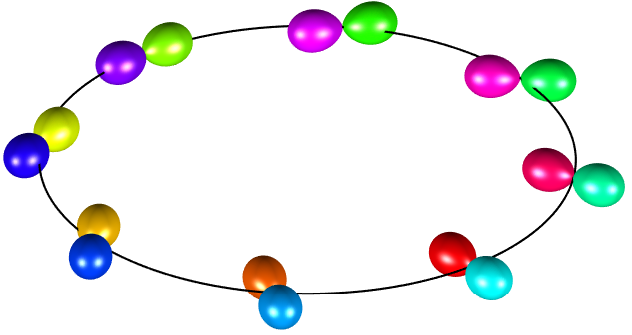
\includegraphics[width=0.45\textwidth]
            {gfx/ch-groundStateSymmetries/polar-HQV.pdf}};
        \node at (7.2, 0) {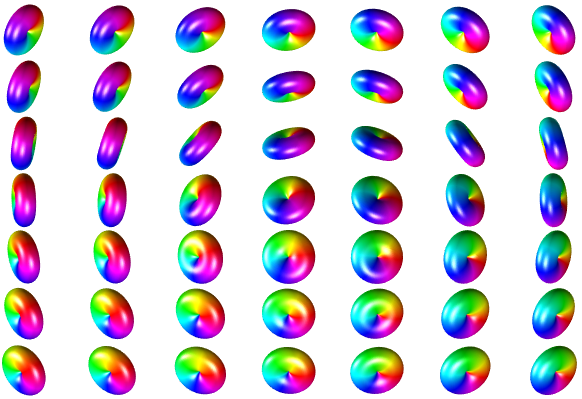
\includegraphics[width=0.45\textwidth]
            {gfx/ch-groundStateSymmetries/coreless.pdf}};
        \node at (-3.6, -0.2) {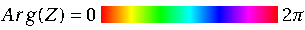
\includegraphics[angle=90]
            {gfx/colourbars/compiled_hsv.pdf}};

        % Labels
        \node at (0, -3) {(a)};
        \node at (7.2, -3) {(b)};
    \end{tikzpicture}
    \caption[Spherical harmonic representation of spin-1 vortices]
    {\label{fig: spin-1-vortices}Spherical harmonic representation of vortices
        in a spin-1 BEC\@.
        (a): Spin-1 polar HQV defined by Eq.~\eqref{eq: polar-HQV}.
        A complete circuit of the vortex results in a \(\pi \) spin rotation of
        the nematic director coupled with a \(\pi \) change to the condensate
        phase.
        (b): Ferromagnetic coreless vortex.
        The vortex takes on a characteristic fountain-like texture of the
        condensate spin vector.}
\end{figure}
By substituting \(\tau=\varphi/2\) in Eq.~\eqref{eq: spinor-superfluid-vel},
and taking \(|\hat{\vb{F}}|=0\) since this is the polar phase, the superfluid
velocity becomes \(\vb{v}_s = \hbar/(2M)\nabla\varphi \).
It immediately follows that the mass circulation is calculated as
\begin{align}
    \oint_C \vb{v}_s \cdot \dd \vb{\ell} = \frac{\kappa}{2},
\end{align}
showing that the unit of circulation is quantised in units of \(\kappa / 2\) for
this system, and hence the name HQV\@.

For the case of the ferromagnetic phase, recall that the first homotopy group is
calculated as~\cite{Kawaguchi2012} \(\pi_1(\mathcal{M}_\text{FM})
= {\mathbb{Z}}_2\), which corresponds to two different classes of line defects:
singular and nonsingular.
The singular vortex configuration can be constructed from
Eq.~\eqref{eq: FM-representative-spinor} using the choice \(\tau'=0\) along with
\(\alpha = \varphi \), which leads to the wave function
\begin{align}
    \psi^\text{FM}_\text{pcv} =
    \sqrt{n}\mqty(
    e^{-i\varphi}\cos^2\frac{\beta}{2} \\
    \frac{1}{\sqrt{2}}\sin\beta \\
    e^{i\varphi}\sin^2\frac{\beta}{2}
    ).
\end{align}
In this configuration, the single-valuedness condition could be satisfied by
having the condensate density vanish along the vortex core.
However, in spinor BECs, we typically have \(c_0 \gg |c_1|\), which implies
that it is more energetically favourable to vary the condensate spin instead.
Therefore, the condensate can instead choose to lift atoms out of the
ferromagnetic state and into the polar state (i.e., occupy the \(m=0\)
component) within the vortex core.
For this reason, such a vortex is referred to as a polar-core
vortex~\cite{Kawaguchi2012}.

An example of a nonsingular vortex arising in the FM phase is the coreless
vortex~\cite{Martikainen2002, Leanhardt2003}, which can be constructed from
Eq.~\eqref{eq: FM-representative-spinor} by choosing \(\tau^\prime = \alpha
= \varphi \) and having \(\beta = \beta(\rho)\) be a function of the transverse
radial coordinate, \(\rho =\sqrt{x^2 + y^2}\), as:
\begin{align}
    \psi^\text{FM}_\text{cl} = \sqrt{n}\mqty(
    \cos^2\frac{\beta}{2} \\
    \frac{e^{i\varphi}}{\sqrt{2}}\sin\beta \\
    e^{2i\varphi}\sin^2\frac{\beta}{2}
    ).
\end{align}
The single-valuedness condition of the wave function is satisfied by choosing
\(\beta(\rho) \) in one of two ways, resulting in slightly different
configurations of a coreless vortex.
If we choose \(\beta(\rho)\) such that \(\beta(\rho=0) = 0\) and
\(\beta(\rho=\rho_0) = \pi/2 \), where \(\rho_0\) is the radius of the system,
then we have what is known as a Mermin-Ho vortex~\cite{Mermin1976,
Mizushima2002a}.
In this configuration, the spin starts aligned with the \(z\)-axis at
\(\rho=0\), then gradually tilts away as \(\rho \rightarrow \rho_0\) until
the spin lies in the \(xy\)-plane at \(\rho=\rho_0\).
A different configuration is obtained if instead one chooses \(\beta(\rho)\)
such that \(\beta(\rho=0) = 0\) and now \(\beta(\rho=\rho_0) = \pi \), leading
to what is known as an Anderson-Toulouse-Chechetkin
vortex~\cite{Chechetkin1976, Anderson1977}.
In this configuration, the spin follows a similar path, but now tilts through
the \(xy\)-plane, and ends up aligned with the \(z\)-axis once more at
\(\rho=\rho_0\), with the spin now pointing in the opposite direction to the
spin at \(\rho=0\).
A spherical harmonic representation of the Mermin-Ho vortex is shown in
Fig.~\ref{fig: spin-1-vortices}b, where the characteristic fountain-like
spin texture is apparent.

\subsection{Vortices in spin-2 systems}\label{sec: vortices-spin-2}
Like the subsection before, we construct a few illustrative examples of vortices
arising in the spin-2 phases and investigate them using spherical harmonics.
We start with the UN phase, as given by
Eq.~\eqref{eq: UN-representative-spinor}.
Unlike the spin-1 polar phase, the UN phase does not support fractional vortices
with mass circulation.
This is apparent from the spherical harmonic representation given in
Fig.~\ref{fig: nematic-graph}a, where the two-fold symmetry
about the \(C_2\) axis is not coupled to the condensate phase, \(\tau \).
This phase instead accommodates a spin vortex, i.e., a vortex which carries only
spin circulation.
Such a vortex is constructed from Eq.~\eqref{eq: UN-representative-spinor} with
the choice \(\tau=0, \alpha=-\varphi/2, \beta=\pi/2\):
\begin{equation}
    \psi^\text{UN}_\text{sv} = \frac{\sqrt{6n}}{4}\mqty(
    e^{i\varphi} \\
    0 \\
    -\sqrt{\frac{2}{3}} \\
    0 \\ e^{-i\varphi}
    ).
\end{equation}
The spherical harmonic representation of this vortex state is shown in
Fig.~\ref{fig: SV-HQV}a.
\begin{figure}
    \centering
    \begin{tikzpicture}
        \node at (0, 0) {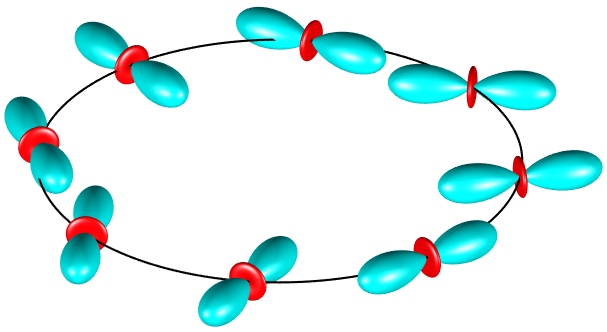
\includegraphics[width=0.45\textwidth]
            {gfx/ch-groundStateSymmetries/UN-spin-vortex.pdf}};
        \node at (7.3, 0) {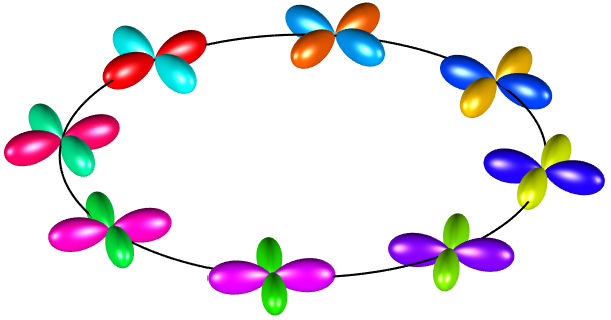
\includegraphics[width=0.45\textwidth]
            {gfx/ch-groundStateSymmetries/BN-HQV.pdf}};
        \node at (3.0, -2) {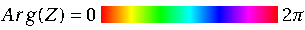
\includegraphics{gfx/colourbars/compiled_hsv.pdf}};

        % Labels
        \node at (-0.8, -2.2) {(a)};
        \node at (7.2, -2.2) {(b)};
    \end{tikzpicture}
    \caption[Spherical harmonic representation of spin-2 vortices]
    {\label{fig: SV-HQV}Spherical harmonic representation of select vortices
    in the spin-2 nematic phases.
    (a): A spin vortex in the UN phase. A complete circuit of the vortex
    results in a \(\pi \) winding of the condensate spin vector, with no
    change to the condensate phase, and hence this vortex has no mass
    circulation.
    (b): One type of half-quantum vortex in the BN phase.
    The condensate phase winds by \(\pi \) about the vortex core which is
    coupled to a \(\pi / 2\) spin rotation.}
\end{figure}
Indeed, we see that as the core of the vortex is traversed, the spin vector
winds by \(\pi \) about the axis perpendicular to the nematic director
(see Fig.~\ref{fig: nematic-graph}a), but the condensate phase remains
unchanged.

Recall that the first homotopy group of the BN phase
(\(\pi_1(\mathcal{M}_\text{BN})=\mathbb{Z} \cross_h
{(\text{D}^*)}_{\hat{\vb{F}}}\)) is non-Abelian, and hence supports non-Abelian
vortices.
Unlike the UN phase, the BN phase can support fractional vortices with mass
circulation.
One such example is of the BN HQV, which, due to the differing first homotopy
group, is topologically distinct from that of the spin-1 polar case
presented in Fig.~\ref{fig: spin-1-vortices}a.
Such a vortex can be constructed from Eq.~\eqref{eq: BN-representative-spinor}
using the choice \(\tau=2\alpha=\varphi/2\) and \(\beta=\gamma=0\):
\begin{equation}
    \psi^\text{BN}_\text{hqv} = \sqrt{\frac{n}{2}}\mqty(
    1 \\
    0 \\
    0 \\
    0 \\
    e^{i\varphi}
    ).
\end{equation}
The spherical harmonic representation of this vortex is shown in
Fig.~\ref{fig: SV-HQV}b.
It is clear this vortex has the typical \(\pi \) phase winding about the vortex
core associated with HQVs, which is also coupled to a \(\pi / 2\) spin rotation.
When a vortex consists of a \(2\pi w\) winding of the condensate phase coupled
to a \(2\pi \sigma\) winding of the spin vector about some axis of symmetry,
the vortex charge can be described as (\(w, \sigma\)).
The particular case of the vortex shown in Fig.~\ref{fig: SV-HQV}b is classed as
a \((1/2, 1/4)\) vortex, where the \(1/2\) and \(1/4\) denote the phase and spin
windings, respectively.
Additionally, there exists a half-quantum spin vortex, also called a
(\(0, 1/2\)) vortex, in this phase, in which the condensate spin winds by
\(\pi \) about the core, but the condensate phase remains
unchanged~\cite{Kawaguchi2012}.

Like the BN phase, the cyclic phase also supports non-Abelian vortices.
Additionally, this phase also supports fractional vortices, but instead of the
half-quantum of circulation that arises in the nematic phases, the cyclic phase
has circulation that is quantised in units of \(\kappa / 3\),
leading to one-third and two-third vortices.
These vortices can be constructed from Eq.~\eqref{eq: general-cyclic-wfn} by
applying a condensate phase and general spin rotation, where a one-third vortex
is constructed from the choice \(\tau = -\alpha = \varphi/3 \) with
\(\gamma = 0\) and a two-third vortex is constructed by choosing
\(\tau = 2\varphi/3\), \(\alpha = \varphi/3\) and \(\gamma=0\).
The result is a phase winding in the \(\psi_2\) and \(\psi_{-1}\) components
for the one-third and two-third vortices, respectively:
\begin{equation}
    \psi^\text{C}_{\frac{1}{3}} = \sqrt{\frac{n}{3}}\mqty(
        e^{i\varphi} \\
        0 \\
        0 \\
        \sqrt{2} \\
        0
    ),
    \qquad
    \psi^\text{C}_{\frac{2}{3}} = \sqrt{\frac{n}{3}}\mqty(1 \\ 0 \\ 0 \\
    \sqrt{2}e^{i\varphi}\\0).
\end{equation}
Spherical harmonic representations are plotted in
Fig.~\ref{fig: cyclic-fractional-spherical}.
\begin{figure}
    \centering
    \begin{tikzpicture}
        \node at (0, 0) {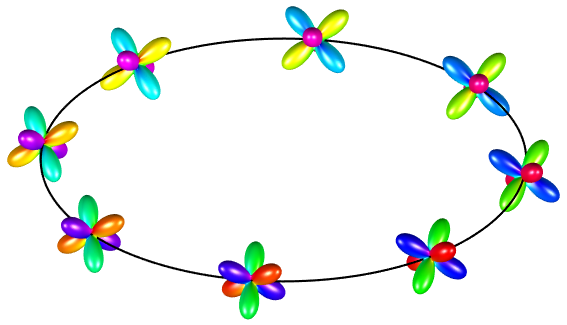
\includegraphics[width=0.45\textwidth]
            {gfx/ch-groundStateSymmetries/one-third-vortex.pdf}};
        \node at (7.3, 0) {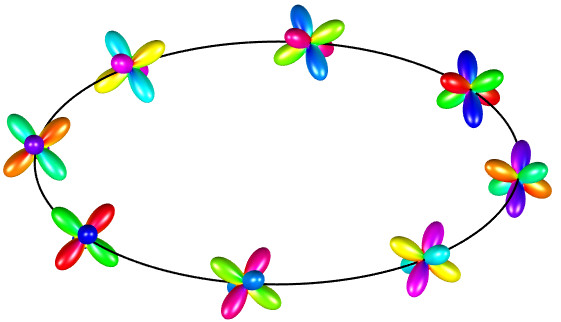
\includegraphics[width=0.45\textwidth]
            {gfx/ch-groundStateSymmetries/two-third-vortex.pdf}};
        \node at (3, -2) {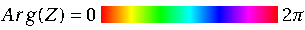
\includegraphics{gfx/colourbars/compiled_hsv.pdf}};

        \node at (0, -2.2) {(a)};
        \node at (7.2, -2.2) {(b)};
    \end{tikzpicture}
    \caption[Spherical harmonic representation of cyclic fractional vortices]
    {\label{fig: cyclic-fractional-spherical}Spherical harmonic
        representations of cyclic fractional vortices.
        (a): A one-third vortex. A complete circuit reveals a \(2\pi/3\)
        winding of the condensate phase, coupled with a \(\pi/2\) spin rotation.
        (b): A two-third vortex. Similarly, a complete circuit of the
        vortex results in a \(4\pi/3\) winding of the condensate phase, again
        coupled to a \(\pi/2\) spin rotation.}
\end{figure}
As we did for the spin-1 HQV in the polar phase, one can use the above wave
function to see that the circulation is now quantised in units of
\(\kappa / 3\).
Substituting \(\tau=\varphi/3\) in Eq.~\eqref{eq: spinor-superfluid-vel}, and
taking \(|\hat{\vb{F}}|=0\) since this is the cyclic phase, the superfluid
velocity becomes \(\vb{v}_s=\hbar/(3M)\nabla\varphi \).
It then immediately follows that the mass circulation is calculated as
\begin{align}
    \oint_C \vb{v}_s \cdot \dd \vb{\ell} = \frac{\kappa}{3},
\end{align}
showing the mass circulation in this phase is quantised in units of
\(\kappa / 3\).